% Dokumentation af PWM-controller %
% UCC1801 %

\section{PWM-controller} \label{PWM}
PWM-controlleren er en vigtig del af en SMPS. Det er den der står for tilpasningen af switch-signalets duty-cycle, således udgangen holdes stabilt, når inputtet påvirkes eller ændres. Det er vigtigt at vælge PWM-controller ud fra kravene til converteren. PWM-controllere er ofte begrænset til en maksimal duty-cycle på enten $50\percent$ eller $100\percent$. Derudover skal der vælges, hvilken form for regulering af converterens udgangstrin der ønskes, da controlleren skal understøtte dette. 

Ud fra beregningerne af den maksimale duty-cycle i afsnit~\ref{maksimum_duty_cycle}, vælges det at PWM-controlleren maksimalt skal have en duty-cycle på $50\percent$. For at kunne opnå en mere præcis regulering, vælges det at bruge peak-current regulering. Denne form for regulering, regulerer efter peak-strømmen i transformatorens primærvikling. Da den regulerer efter dette, opnås der også en strømbegrænser i regulerings-loopet. Ud fra disse krav vælges en PWM-controller af typen UCC1801\cite{UCC1801}. Det er en controller Terma har erfaring med, og derfor også nemt kan udskiftes med en space-godkendt controller.

På figur~\ref{fig:PWM_block_diagram} ses et funktionelt block diagram over UCC1801. Det indeholder controllerens overordnede komponenter, og giver et overblik over dens funktionalitet. 

\begin{figure}[H]
	\center
	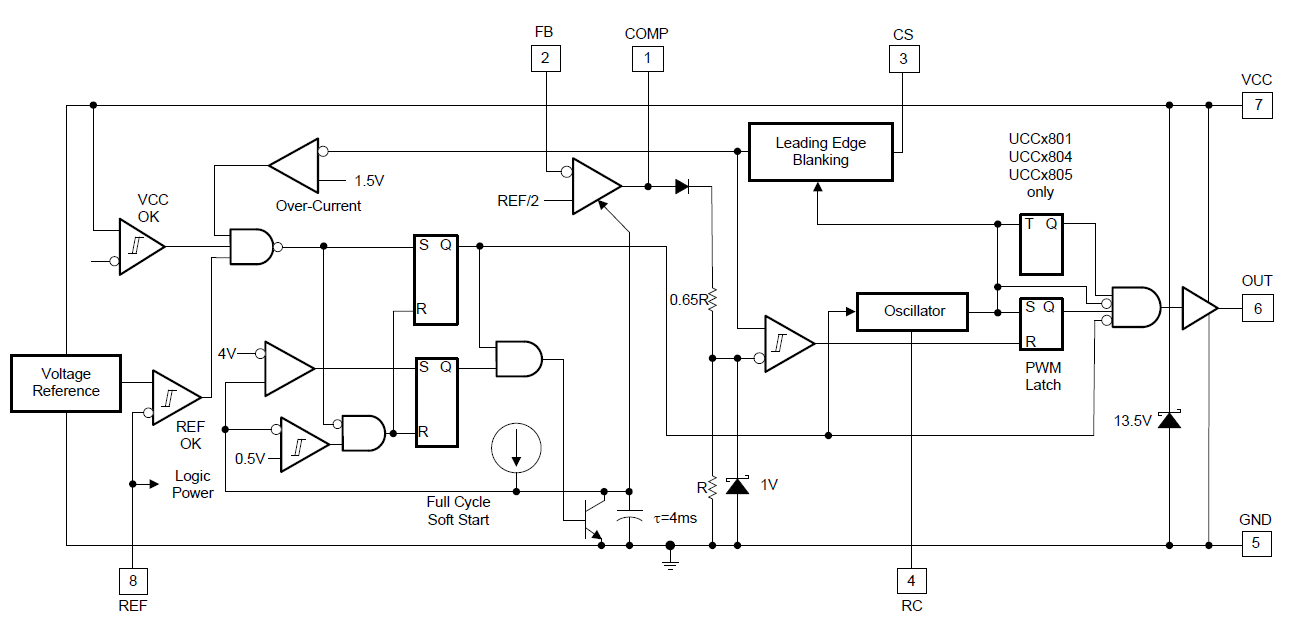
\includegraphics[max width=0.9\linewidth]{/tex/2iteration/billeder/PWM_block_diagram.PNG}
	\caption{UCC1801 - Funktionelt Block Diagram}
	\label{fig:PWM_block_diagram}
\end{figure}

Tabel~\ref{tab:ucc1801_specs} viser de mest essentielle specifikationer for UCC1801, i forhold til en flyback converter. Disse er udvalgte specifikationer fra databladet.

\begin{table}[H] 			
	\centering
	\begin{tabularx}{\textwidth}{|X|c|c|c|} 
		\hline
		\textbf{Specifikation} & \textbf{Min} & \textbf{Typ} & \textbf{Max} \\ \hline
		$V_{CC}$ &  &  & $12V$ \\ \hline
		$I_{out}$ &  &  & $1A$ \\ \hline
		$V_{Reference}$ & $4.925V$ & $5V$ & $5.075V$ \\ \hline
		$D_{max}$ & $48\percent$ & $49\percent$ & $50\percent$ \\ \hline
		$V_{on,th}$ & $8.6V$ & $9.4V$ & $10.2V$ \\ \hline
		$V_{off,th}$ & $6.8V$ & $7.4V$ & $8V$ \\ \hline
		Temperature Range & $-55\degreeCelsius$ &  & $125\degreeCelsius$ \\ \hline
		$f_{osc}$ & & & $1M\hertz$ \\ \hline
	\end{tabularx}

	\caption{Relevante specifikationer for UCC1801}
	\label{tab:ucc1801_specs}
\end{table}

Der tages udgangspunkt i en UCC1801, med en PDIP pakke type. Figur~\ref{fig:ucc1801_pin_overview} viser en oversigt over ben konfigurationen for en sådan pakke. Det er en 8-bens IC, hvor samtlige ben bliver brugt. Benenes funktionalitet er overordnet beskrevet i tabel~\ref{tab:ucc1801_pin_functionality}, og vil blive uddybet i de følgende afsnit.

\begin{figure}[H]
	\center
	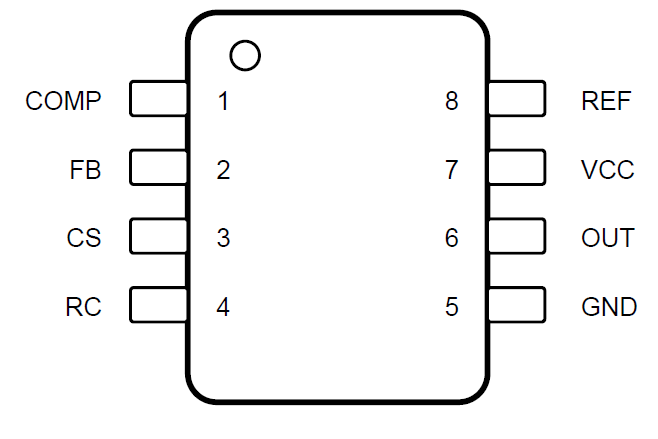
\includegraphics[max width=0.7\linewidth]{/tex/2iteration/billeder/ucc1801_pin_overview.PNG}
	\caption{Ben konfiguration for UCC1801}
	\label{fig:ucc1801_pin_overview}
\end{figure}

\begin{table}[H] 			
	\centering
	\begin{tabularx}{\textwidth}{|c|c|c|X|} 
		\hline
		\textbf{Navn} & \textbf{Ben} & \textbf{I/O} & \textbf{Beskrivelse} \\ \hline
		COMP & 1 & O & COMP er outputtet fra den indbyggede fejlforstærker. Dette ben bruges til at lave et feedback til FB benet i reguleringssløjfen. 	\\ \hline
		FB 	 & 2 & I & FB er inputtet til den indbyggede fejlforstærker. Den er forbundet til den inverterende indgang af forstærkeren. Den bruges sammen med COMP, som en del af reguleringssløjfen.\\ \hline
		CS   & 3 & I & CS er inputtet til current sense komparatorne. UCC1801 har to komparatorerne til current sense: PWM komparatoren og overstrøms komparatoren. PWM-komparatoren bruges til, at trække udgangssignalet lavt, når CS-signalet overstiger $1V$. Overstrøms komparatoren er en indbygget overstrømsbeskyttelse. Den tvinger udgangen lav, så længe CS-signalet er over $1.5V$ \\ \hline
		RC 	 & 4 & I & RC er inputtet til oscillatoren. Oscillatorfrekvensen, og dermed også switch-frekvensen, sættes ud fra tidskonstanten mellem en modstand og en kondensator.  \\ \hline
		GND  & 5 & - & GND er ground for IC'ens komponenter.  \\ \hline
		OUT  & 6 & O & OUT er IC'ens output. Det er et PWM-signal, hvis duty-cycle afhænger af PWM-komparatoren. Outputtet skiftes mellem GND og VCC, hvilket betyder at VCC skal være høj nok, til at drive MOSFET'en.  \\ \hline
		VCC  & 7 & I & VCC er forsyning til IC'ens komponenter. Det foreslås at vælge en høj VCC, for at mindske støjpåvirkninger. For at mindske støj på forsyningen anbefales det, at bypasse VCC med en kondensator på minimum $1\micro \farad$, tæt på IC'en. \\ \hline
		REF  & 8 & O & REF er outputtet for IC'ens interne spændingsreference. Den bruges bl.a. som reference til fejlforstærkeren. Derudover forsyner den IC'ens logiske komponenter. For at mindske støj på referencen, anbefales det at bypasse REF med en kondensator på minimum $1\micro \farad$, tæt på IC'en. \\ \hline
	\end{tabularx}
	
	\caption{Ben funktionalitet for UCC1801}
	\label{tab:ucc1801_pin_functionality}
\end{table}

\subsection{Under Voltage LockOut}
UCC1801 indeholder en Under Voltage LockOut (UVLO) beskyttelse. Dette betyder, at forsyningsspændingen skal være et bestemt niveau, før controlleren starter. Som en konsekvens af dette vil både output og referencespændingen holdes lav, indtil grænseværdien er nået. For at have en hysteresemargin, har den både et turn ON og et turn OFF niveau. Ved UCC1801 er disse niveauer $V_{on,th}=9.4V$ og $V_{off,th}=7.4V$. Da amplituden af output-signalet er lig VCC, vil controlleren ikke prøve at drive MOSFET'en før $V_{CC}=9.4V$. Da en MOSFET typisk har en $V_{gs,th}$ mellem $4$ og $5V$, vil der ikke opnås et stadie hvor MOSFET'en kun er delvist ON. Dette ses også på referencespændingen, da den først bliver $5V$ når $V_{CC}\geqslant 9.4V$. Referencen kan derfor også bruges, som en ON/OFF indikator. 

\subsection{Switch-frekvens}
Controllerens switch-frekvens sættes af oscillatorblokken i block diagrammet. Den genererer en savtand-spænding, som trigger den efterfølgende latch. Dette giver et PWM-signal, da det skifter mellem VCC og GND.
Stigetiden for savtand spændingen bliver bestemt af tidskonstanten for et eksternt RC-kredsløb. Faldetiden for signalet bliver bestemt af den eksterne kondensator, samt ON-modstanden i en intern transistor. Den on-modstand er opgivet til ca. $130\ohm$. Denne faldetid vil begrænse den maksimale duty-cycle, da outputtet vil være lavt i løbet af faldetiden. 

\begin{figure}[H]
	\center
	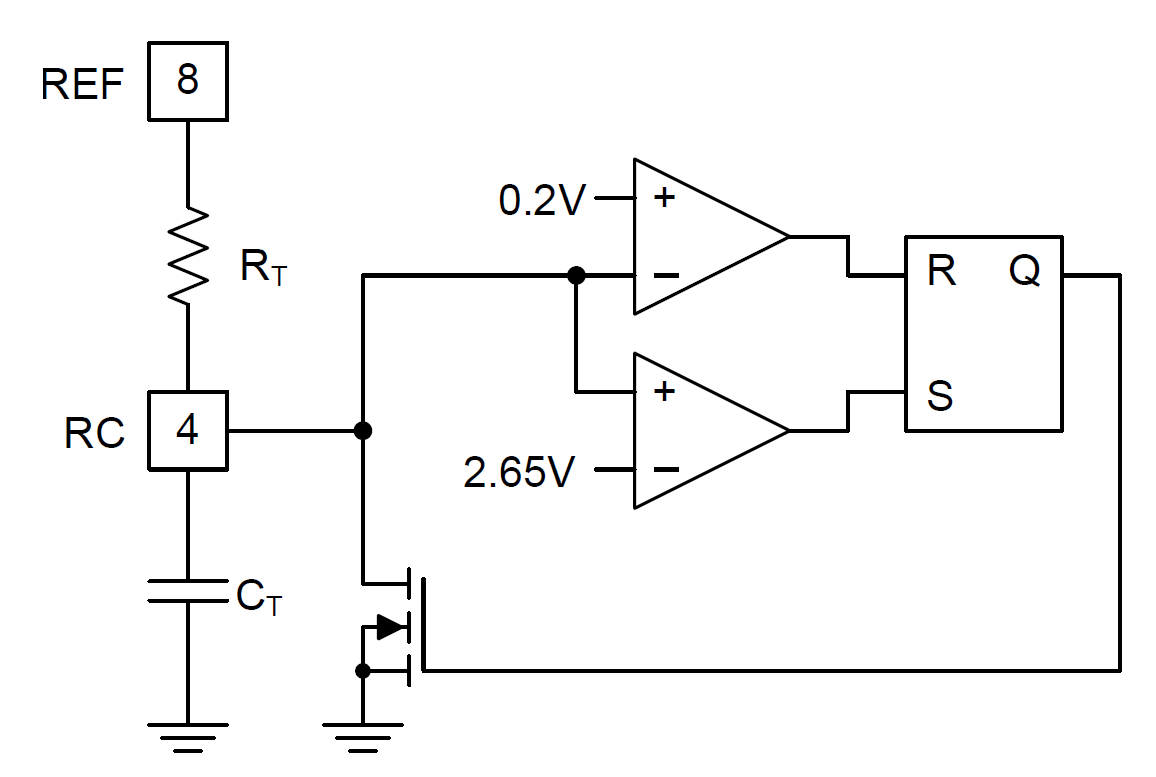
\includegraphics[max width=0.7\linewidth]{/tex/2iteration/billeder/PWM_oscillator_diagram.PNG}
	\caption{Oscillator diagram}
	\label{fig:PWM_oscillator_diagram}
\end{figure}

Figur~\ref{fig:PWM_oscillator_diagram} viser et ækvivalent diagram for oscillator blokken. Komponenterne $R_T$ og $C_T$ er det eksterne RC kredsløb, mens resten er interne komponenter. På diagrammet ses det, at operationsforstærkerne er koblet til henholdsvis $0.2V$ og $2.65V$. Dette sætter maksimum og minimum for savtand spændingen. 

Da der skal komme en flanke på output-signalet hver gang savtand spændingen rammer maksimum, skal frekvensen af savtand spændingen være den dobbelte af den ønskede switch-frekvens. Der ønskes en switch-frekvens på $100k\hertz$, derfor sættes oscillator frekvensen til $f_{osc}=200k\hertz$. I databladet er det anbefalet at $R_T$ vælges mellem $10k\ohm$ og $200k\ohm$, mens det anbefales at $C_T$ vælges mellem $100p\farad$ og $1000p\farad$. Formel~\ref{f_osc} er opgivet i databladet og bruges til at estimere RC komponenterne. $C_T$ sættes til $200p\farad$, og $R_T$ beregnes:
\begin{equation} \label{f_osc}
R_{T} = \frac{1.5}{f_{osc} \cdot C_T} = \frac{1.5}{f_{osc} \cdot C_T} = 37.5k\ohm
\end{equation}
Ved et opslag i databladet ses det, at med en $C_T=200p\farad$ kan der maksimalt opnås en duty-cycle på ca. $48.9\percent$. Da converteren maksimalt skal opererer med en duty-cycle på $44.7\percent$, godtages dette.

\subsection{Current sense kredsløb} \label{CS_loop}
Som nævnt i afsnit~\ref{PWM} er der valgt at bruge peak-current regulering. Denne form for regulering består af to reguleringssløjfer - en spændings- og en strømsløjfe. I dette afsnit beskrives dimensioneringen af strøm sløjfen, mens spændingssløjfen beskrives i afsnit~\ref{V_loop}.

Current sense kredsløbet består, som minimum, af en current sense modstand. Denne modstand bruge til at konvertere strømmen i transformatorens primærvikling om til en spænding. Denne konvertering vil gøre, at kurveformen for strømmen og spændingen er ens, dog med en faktor til forskel. PWM-komparatoren i controlleren trigger udgangen, når current sense spændingen er rampet op til $1V$. Derfor skal modstanden dimensioneres således, spændingen over den er lig $1V$ når peak-strømmen i transformatoren er lig $5.53A$. Dette regnes ud fra Ohm's lov:
\begin{equation} \label{R_cs}
R_{cs} = \frac{1V}{5.53A} = 0.181\ohm
\end{equation}

Da den mindste modstandsværdi der er til rådighed er på $1\ohm$, vil der blive brugt $6\cdot 1\ohm$ i parallel. Dette vil give en modstandsværdi på $0.167\ohm$. Med dette vil strømmen blive delt i de seks modstande, som derved deler den samlede effekt mellem sig. Da der benyttes $0,5W$ modstande, vil dette samtidig gøre, at de ikke brænder af. 

Når current-sense modstanden vælges mindre end den ideelle værdi, vil det tillade en større peak-strøm i primærviklingen. Det regnes ud fra ovenstående forhold til ca. $6A$. Der vil dog stadig i beregninger blive benyttet peak-strømmen på $5.53A$.



\subsubsection{Filtrering}
\noindent På grund af switching-spikes i MOSFET'en, når den går ON, vil der også komme spikes på current sense signalet. Hvis disse spikes når et niveau der er højere end $1V$, vil det trigge komparatoren. Dette vil få controlleren til at generer et PWM-signal, der er meget lavere end det ønskede. Derfor implementeres der et filter, for at filtrere disse spikes væk.

UCC1801 har et indbygget digitalt filter, kaldet Leading Edge Blanking. Dette filter er designet til at filtrere de første $100ns$ af signalet væk, og dermed fjerne spiken. Ideelt set vil dette give et signal, som ses på figur~\ref{fig:ucc1801_leading_edge}.

\begin{figure}[H]
	\center
	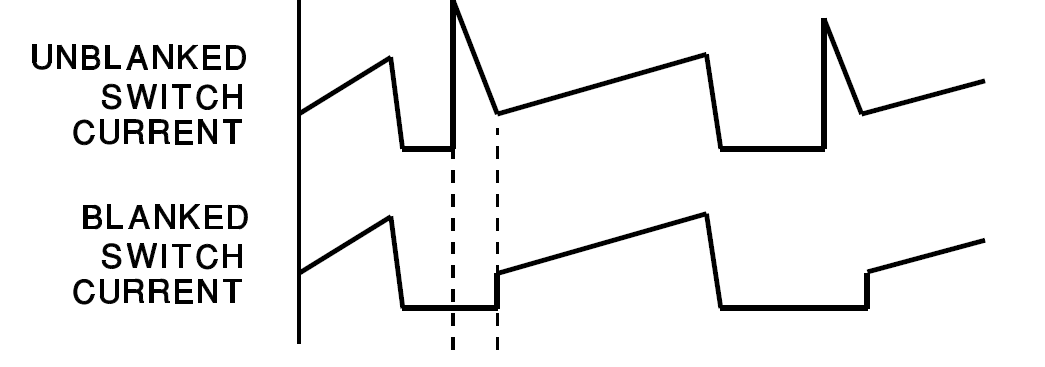
\includegraphics[max width=0.7\linewidth]{/tex/2iteration/billeder/ucc1801_leading_edge.PNG}
	\caption{Current sense signal før og efter Leading Edge Blanking}
	\label{fig:ucc1801_leading_edge}
\end{figure}

\noindent Det digitale filter er ikke altid tilstrækkeligt, og derfor designes et eksternt analogt RC-filter, for yderligere filtrering. Det designes til at have en stigetid på $300ns$, for at tilføje en yderligere filtrering på ca. $200ns$ i forhold til det digitale filter. 

\noindent Med en stigetid på $300ns$, kan båndbredden af filteret estimeres\cite{risetime}:
\begin{equation} \label{filter_BW}
BW \approx \frac{0.34}{t_r} \approx 1.133M\hertz
\end{equation} 

\noindent Der vælges en kondensator på $C_f=100pF$. Ud fra kondensatoren og den ønskede båndbredde i filteret, regnes modstanden.
\begin{equation} \label{filter_R}
R_f = \frac{1}{2 \cdot \pi \cdot BW \cdot C_f} = \frac{1}{2 \cdot \pi \cdot 1.133M\hertz \cdot 100pF} = 1.4k\ohm
\end{equation}

\noindent Med det designede filter vil stigetiden af current sense signalet nu blive begrænset af filteret. Derfor vil den første del af signalet ligne et første ordenssystem, der stiger indtil spændingen når det niveau, der svarer til strømmen i primærviklingen. Derefter vil signalet stige som en ret linje, ligesom strømmen. Dette ses på figur~\ref{fig:ucc1801_CS_filter}, hvor det øverste signal er før filteret, og det nederste er efter.

\begin{figure}[H]
	\center
	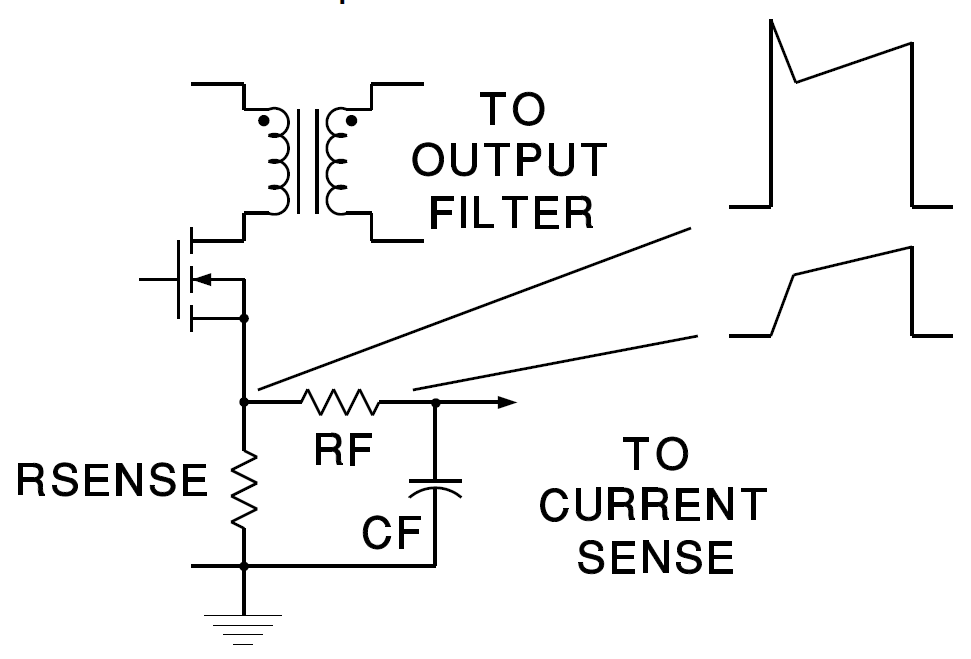
\includegraphics[max width=0.7\linewidth]{/tex/2iteration/billeder/ucc1801_CS_filter.PNG}
	\caption{Current sense signal før og efter eksternt RC-filter}
	\label{fig:ucc1801_CS_filter}
\end{figure}

\subsubsection{Overstrømsbeskyttelse} \label{CS_protection}
\noindent En fordel ved at regulere efter strømmen i transformatoren er, at der opnås en overstrømsbeskyttelse. Når strømmen stiger, vil PWM-controlleren sænke duty-cyclen, og derved også sænke udgangsspændingen. Dette giver en I/V karakteristik der, ideelt set, er næsten firkantet. Dette er skitseret på figur~\ref{fig:I-V_karateristik}. 

\begin{figure}[H]
	\center
	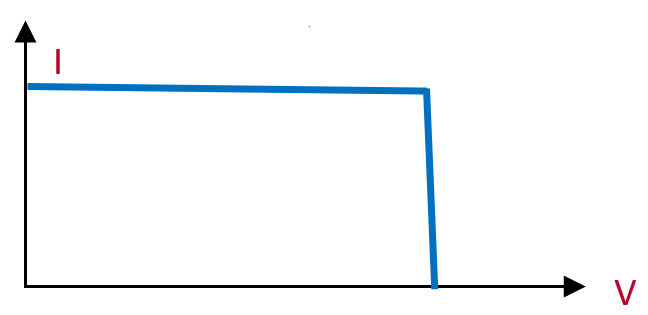
\includegraphics[max width=0.7\linewidth]{/tex/2iteration/billeder/I-V_karakteristik.PNG}
	\caption{I/V karakteristik for converteren}
	\label{fig:I-V_karateristik}
\end{figure}

\noindent Denne karakteristik kan dog ikke opnås i realiteten. Filteret der er indsat for at filtrere current sense signalet, vil lave en hale på karakteristikken. Det sker fordi controlleren ikke ser den faktiske strøm, men den filtrerede, når duty-cyclen er lav. 

Da det er nødvendigt at filtrere current sense signalet for at reguleringen fungerer, kan filtrets påvirkning af I/V karakteristikken ikke undgås. Til gengæld kan filtret optimeres, således at det kun lige akkurat filtrerer nok, og på den måde skader I/V karakteristikken mindst muligt. Denne optimering vil ske i 3. iteration. 

\subsection{Spændingsregulering} \label{V_loop}
I dette afsnit beskrives spændingssløjfen. Den består hovedsageligt af to dele: en spændingsdeler og en fejlforstærker. Spændingsdeleren deler udgangsspændingen ned, så den ønskede udgangsspænding er lig en intern reference i IC'en. Fejlforstærkeren står for selve reguleringen. Den inverterende indgang og udgangen på fejlforstærkeren er ført ud, således det er muligt at indsætte et kompenseringsnetværk.

Figur~\ref{fig:regulerings_blokdiagram} viser et blokdiagram for reguleringssløjfen. Det viser de to overføringsfunktioner, der bruges til at modulere systemet. Forstærkningen i fejlforstærkeren er trukket ud af blokken for overføringsfunktionen, da det er produktet mellem forstærkningen i spændingsdeleren og fejlforstærkeren, der giver reguleringssløjens samlede forstærkning. 

\begin{figure}[H]
	\center
	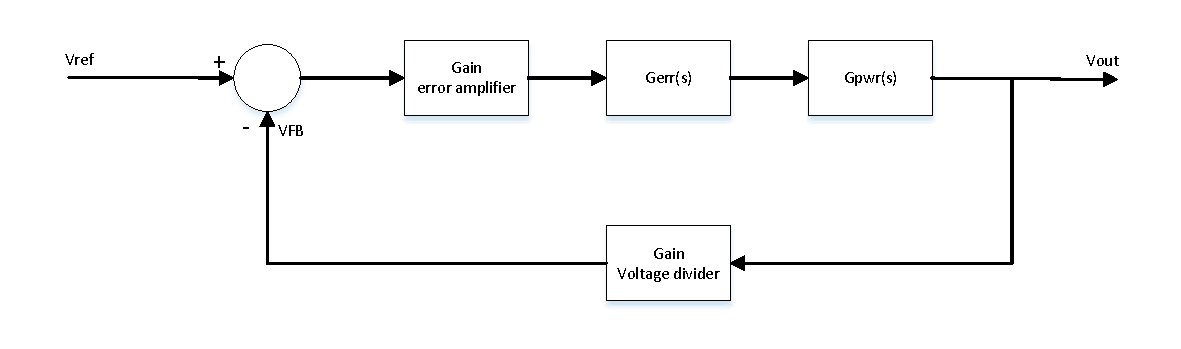
\includegraphics[max width=0.7\linewidth]{/tex/2iteration/billeder/Regulerings_blokdiagram.pdf}
	\caption{Reguleringsblokdiagram}
	\label{fig:regulerings_blokdiagram}
\end{figure}

\subsubsection{Spændingsdeler}
Den ikke inverterende indgang på den indbyggede fejlforstærker i UCC1801, er forbundet til den halve reference spænding, dvs. $2.5V$. Derfor skal der designes en spændingsdeler, der deler den ønskede udgangsspænding på $21V$ ned til $2.5V$. Figur~\ref{fig:Voltagedivider_ideal} viser kredsløbet for spændingsdeleren. 

\begin{figure}[H]
	\center
	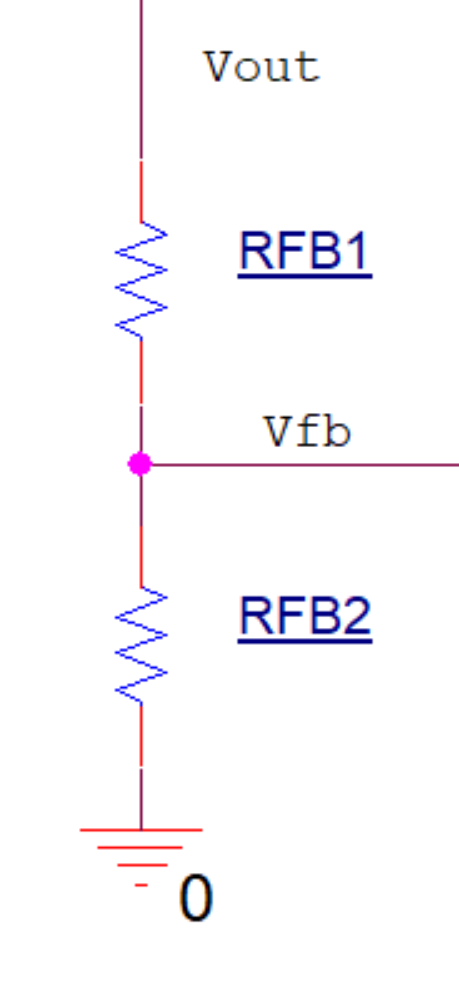
\includegraphics[max width=0.7\linewidth]{/tex/2iteration/billeder/Voltagedivider_ideal.PNG}
	\caption{Spændingsdeler diagram}
	\label{fig:Voltagedivider_ideal}
\end{figure}

Spændingsdeleren designes således der løber en strøm på $1mA$ i den. Derved påvirker den ikke udgangsstrømmen. Derudover dimensioneres de to modstande, således der er et spændingsfald på $2.5V$ over $R_{FB2}$, og $21V-2.5V$ over $R_{FB1}$. $R_{FB1}$ er beregnet med ligning~\ref{RFB1}.

\begin{equation} \label{RFB1}
R_{FB1} = \frac{V_{out}-V_{FB}}{I_{FB1}} = \frac{21V-2.5V}{1mA} = 18.5k\ohm
\end{equation}

\noindent $R_{FB2}$ er beregnet ud fra spændingsdeler formlen, ligning~\ref{RFB2}. Her løses $R_{FB2}$, og fås til $R_{FB2}=2.527k \ohm$.  
\begin{equation} \label{RFB2}
V_{FB} = \frac{R_{FB2}}{R_{FB1} + R_{RB2}} \cdot V_{out}
\end{equation}

For at opnå en præcis spændingsdeler vælges der at bruge to modstande i parallel. Den ene modstand vælges til $R_{FB21}=2.55k\ohm$. Mens den anden regnes ud fra den ønskede samlede modstandsværdi. Dette gøres ved ligning~\ref{RFB22}, som løses med hensyn til $R_{FB22}$. Dette giver $R_{FB22}=280.5k\ohm$, som afrundes til $280k\ohm$.
\begin{equation} \label{RFB22}
R_{FB2} = ((R_{FB21})^{-1} + (R_{FB22})^{-1})^{-1}
\end{equation}

\subsubsection{Fejlforstærker}
Som en del af reguleringen opstilles der først en overføringsfunktion for power-modulet. Denne overføringsfunktion er opgivet i databladet for UCC1801, og er skrevet ved ligning~\ref{H_Power}.
\begin{equation} \label{H_Power}
G_{pwr}(s) = G_0 \cdot \frac{(1+\frac{s}{2\pi \cdot f_{ESRz}}) \cdot (1-\frac{s}{2\pi \cdot f_{RHPz}})}{1+\frac{s}{2\pi \cdot f_{p1}}} \cdot \frac{1}{1 + \frac{s}{2\pi \cdot f_{p2}} + \frac{s^2}{(2\pi \cdot f_{p2})^2}}
\end{equation}

Overføringsfunktionen består af flere dele: en DC-forstærkning, to poler og to nulpunkter. DC-forstærkningen, $G_0$, er skrevet ved ligning~\ref{DC_gain}. Den er især bestemt af belastningen, current sense kredsløbet, transformatoren og switch-frekvensen. Den regnes til en forstærkning på $10.74$ gange, eller $20.6\decibel$.
\begin{equation} \label{DC_gain}
G_0 = \frac{R_{out} \cdot N}{R_{CS} \cdot A_{CS}} \cdot \frac{1}{\frac{(1-D)^2}{\tau_L} + (2 \cdot M) + 1} = 10.7gg \Rightarrow 20.6\decibel
\end{equation}
\noindent Hvor:
\newline \noindent $N$ er omsætningsforholdet i transformatoren.
\newline \noindent $A_{CS}$ er den interne forstærkning i current sense kredsløbet, og aflæses i databladet til $1.65$.
\newline \noindent $D$ er den maksimale duty-cycle, som er $0.447$.
\newline \noindent $\tau_L$ er converterens tidskonstant. Den regnes ud fra ligning~\ref{tau_L}.
\begin{equation} \label{tau_L}
\tau_L = \frac{2 \cdot L_P \cdot f_s}{R_{out} \cdot N^2}
\end{equation}
\newline \noindent $M$ er spændingsomsætningen fra indgang til udgang. Den regnes ud fra ligning~\ref{M}.
\begin{equation} \label{M}
M = \frac{V_{out} \cdot N}{V_{in}}
\end{equation}

En flyback converter, som opererer i CCM, har to primære nulpunkter der kan påvirke stabiliteten i systemet. Det er også de to nulpunkter, der er inkluderet i overføringsfunktionen. Den ene, $f_{ESRz}$, er bestemt af produktet mellem udgangskapaciteten og den indre seriemodstand i udgangskondensatoren. Placeringen af denne er regnet ved ligning~\ref{ESR_zero}.
\begin{equation} \label{ESR_zero}
f_{ESRz} = \frac{1}{2 \cdot \pi \cdot R_{ESR} \cdot C_{out}} = 189.5k\hertz
\end{equation}

\noindent Det andet nulpunkt er højre-halvplans-nulpunktet. Det er ofte dette nulpunkt, der er det dominerende af de to, og derfor den der skal tages højde for i reguleringen. Placeringen af dette er regnet ved ligning~\ref{RHP_zero}. Placeringen af dette nulpunkt, er afhængigt af størrelsen på belastningen, samt inputspændingen. Placeringen stiger ved højere inputspændinger, og mindre belastninger. 
\begin{equation} \label{RHP_zero}
f_{RHPz} = \frac{R_{out} \cdot (1-D)^2 \cdot N^2}{2 \cdot \pi \cdot L_P \cdot D} = 15.8k\hertz
\end{equation}

\noindent Ud fra ligning~\ref{ESR_zero} og \ref{RHP_zero}, ses det, at det er højre-halvplans nulpunktet der er det dominerende nulpunkt i converteren. Når båndbredden skal vælges, er det derfor vigtigt, at den ligger tilpas meget lavere end det dominerende nulpunkt.

Converteren har også to relevante poler. Den dominerende pol bestemmes af loaden og udgangskondensatoren. Den anden pol er placeret ved den halve switching-frekvens. De to poler er beregnet ved ligning~\ref{pol1} og \ref{pol2}.
\begin{equation} \label{pol1}
f_{p1} = \frac{\frac{(1-D)^3}{\tau_L} + 1 + D}{2\cdot \pi \cdot R_{out} \cdot C_{out}} = 132.8\hertz
\end{equation}

\begin{equation} \label{pol2}
f_{p2} = \frac{f_s}{2} = 50k\hertz
\end{equation}

\noindent Bode plottet for power-modulet plottes i MATLAB på figur~\ref{fig:MATLAB_power_module}. Her aflæses DC-forstærk-ningen til $20.6\decibel$. Derudover aflæses der en pol ved ca. $130\hertz$ og ved ca. $50k\hertz$. Dette stemmer overens med de beregnede værdier.

Konsekvensen af højre-halvplans nulpunktet ses også tydeligt på figur~\ref{fig:MATLAB_power_module}. Når frekvensen nærmer sig nulpunktet bliver forstærkningen øget med $20 \decibel$/decade, som ved et venstre-halvplans nulpunkt. Tilgengæld vil fasen blive trukket ned med $90^\circ$, i stedet for op. Da polen fra switch-frekvensen ligger ca. samme sted, og også trækker fasen ned med $90^\circ$, kommer der et stort fasedrej i dette frekvensområde. Det kan gøre systemet ustabilt hvis gain-marginen ikke er tilstrækkelig stor. 

\begin{figure}[H]
	\center
	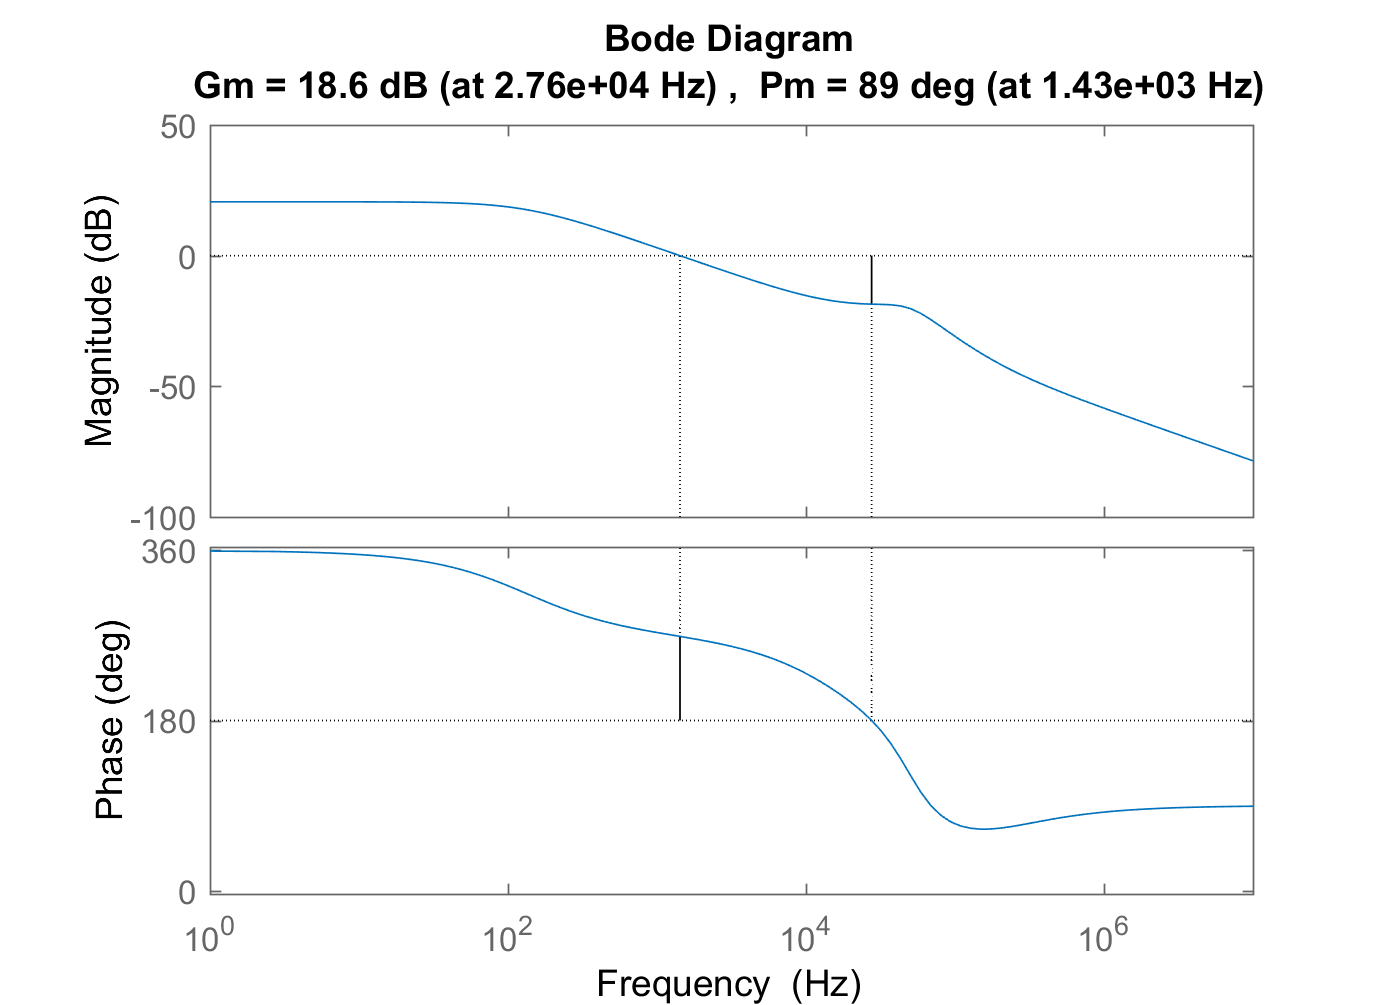
\includegraphics[max width=0.7\linewidth]{/tex/2iteration/billeder/MATLAB_power_module.PNG}
	\caption{Bode plot for power-modulet}
	\label{fig:MATLAB_power_module}
\end{figure}

\noindent I denne iteration designes der et kompensationsnetværk, der vil sikre et stabilt system, med en lav båndbredde. Dette vil blive optimeret i en senere iteration. 
Da der ønskes en lavere båndbredde, end det converteren har i forvejen, indsættes et RC-led i serie som kompensationsnetværk. Ved at bruge et RC-led, vil kondensatoren bestemme forstærkningen ved lave frekvenser, fordi impedansen her er stor. Mens modstanden vil bestemme forstærkningen ved høje frekvenser, fordi kondensatoren vil blive set som en kortslutning. 

Den endelige båndbredde af systemet ønskes på ca. $800\hertz$. Det vil sikre, at systemet ikke bliver ustabilt. For at opnå den ønskede båndbredde aflæses det ud fra bode plottet på figur~\ref{fig:MATLAB_power_module}, at forstærkningen skal mindskes med ca. $5.4\decibel$, eller ca. $0.535GG$, ved frekvenser over $800\hertz$. Den samlede forstærkning af reguleringssløjfen, bestemmes af produktet mellem forstærkningen i spændingsdeleren og forstærkningen i fejlforstærkeren. Forstærkningen i spændingsdeleren regnes ved ligning~\ref{voltagedivider_gain}.
\begin{equation} \label{voltagedivider_gain}
g_{FB} = \frac{R_{FB2}}{R_{FB1}+R_{FB2}} = 0.12
\end{equation}

\noindent Nu kan feedback modstanden i fejlforstærkeren regnes ved ligning~\ref{error_opamp_gain}. 
\begin{equation} \label{error_opamp_gain}
g_{tot} = \frac{R_{comp}}{R_{par}} \cdot g_{FB}
\end{equation}

\noindent Hvor:
\newline \noindent $g_{tot}$ er det ønskede gain i fejlforstærkeren, som er $g_{tot}=0.535gg$.
\newline \noindent $R_{comp}$ er feedback modstanden i fejlforstærkeren, som ønskes dimensioneret.
\newline \noindent $R_{par}$ er parallelmodstanden mellem $R_{FB1}$ og $R_{FB2}$. Den regnes til $R_{par}=2.244k\ohm$.

\noindent De kendte værdier indsættes og ligningen løses for $R_{comp}$. Den fås til $R_{comp}\approx 10k\ohm$.


\noindent For at sikre den lave båndbredde, sættes knækfrekvensen på integratoren til $f_0=300\hertz$. Dermed sikres det, at fejlforstærkeren dæmper signalet ved den ønskede båndbredde på $800\hertz$. Nu kan den tilhørende kapacitet regnes, ud fra $R_{comp}$ og $f_0$.
\begin{equation} \label{c_comp}
c_{comp} = \frac{1}{2\cdot \pi \cdot R_{comp} \cdot f_0} \approx 50nF
\end{equation}

\noindent Med afrundede komponentværdier, regnes den nye knækfrekvens for fejlforstærkeren.
\begin{equation} \label{f_0}
f_0 = \frac{1}{2\cdot \pi \cdot R_{comp} \cdot c_{comp}} = 318.3\hertz
\end{equation}

\noindent Overføringsfunktionen for fejlforstærkeren kan nu opskrives ved ligning~\ref{H_err}.
\begin{equation} \label{H_err}
G_{err}(s) = (\frac{318.3\hertz \cdot 2\cdot\pi}{s} + 1) \cdot 0.535
\end{equation}

\noindent Den plottes i MATLAB, som et bodeplot på figur~\ref{fig:MATLAB_error_op_amp_2}. Her ses det, at den ønskede funktion af integratoren er opnået. På grund af kondensatoren, har den et stort gain ved lave frekvenser. Forstærkningen ligger derimod konstant ved ca. $-5.4\decibel$, efter den ønskede knækfrekvens på ca. $318\hertz$.

\begin{figure}[H]
	\center
	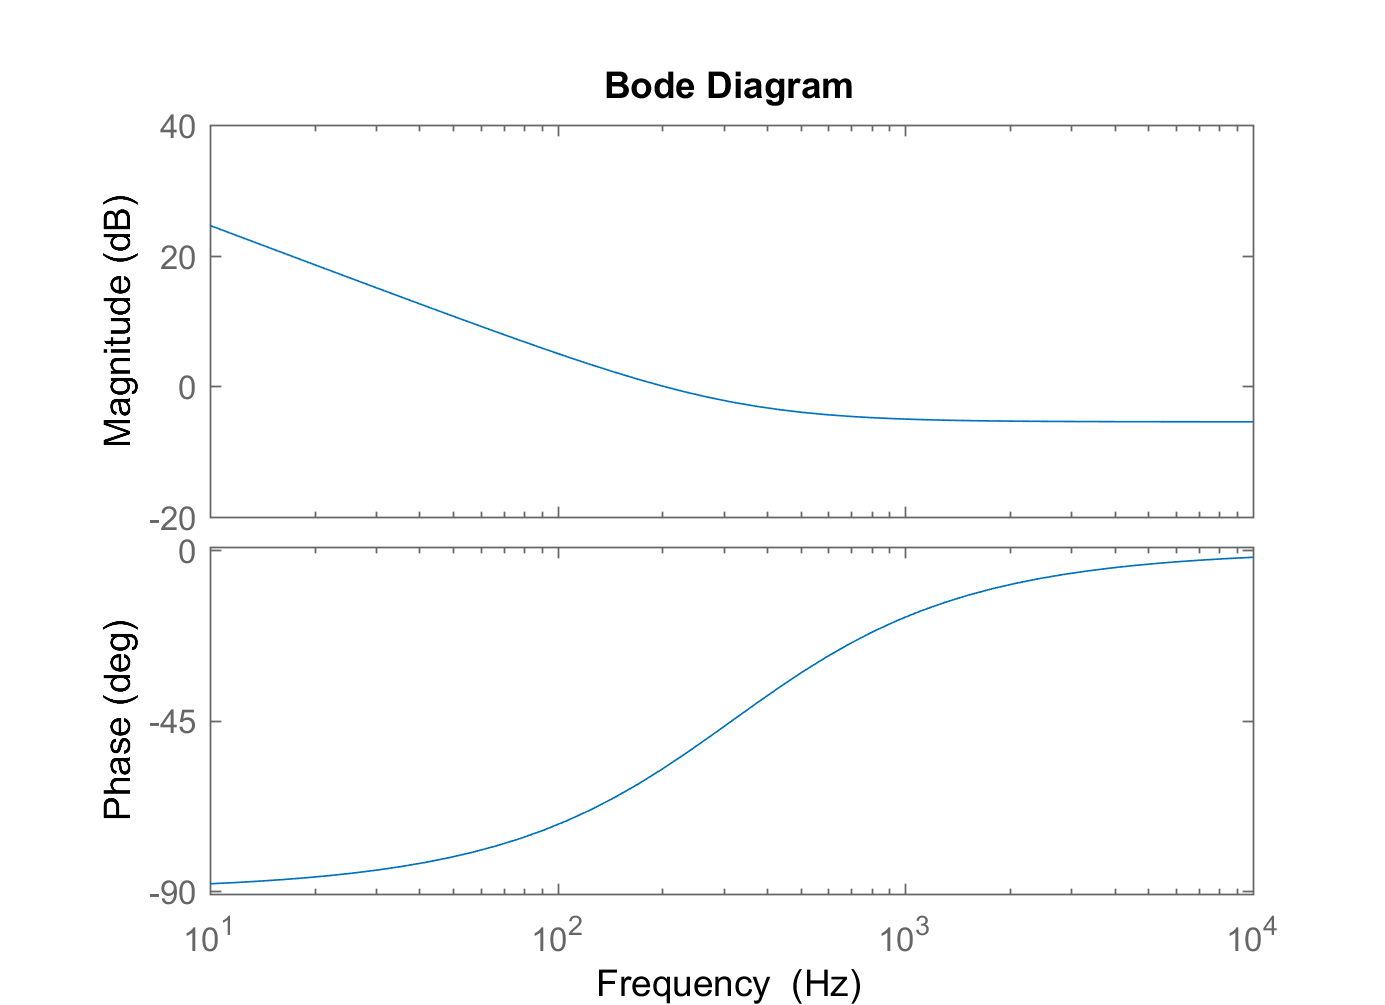
\includegraphics[max width=0.7\linewidth]{/tex/2iteration/billeder/MATLAB_error_op_amp.PNG}
	\caption{Bode plot for fejlforstærker}
	\label{fig:MATLAB_error_op_amp_2}
\end{figure}

\noindent De to overføringsfunktioner ganges sammen, for at bestemme den samlede overføringsfunktion for converteren. Figur~\ref{fig:MATLAB_total_2} viser et åben sløjfe bodeplot af det. Det aflæses at converteren vil have en båndbredde på $810\hertz$. Derudover aflæses fase-margin til $74.3^\circ$, og gain-margin til $24\decibel$.

\begin{figure}[H]
	\center
	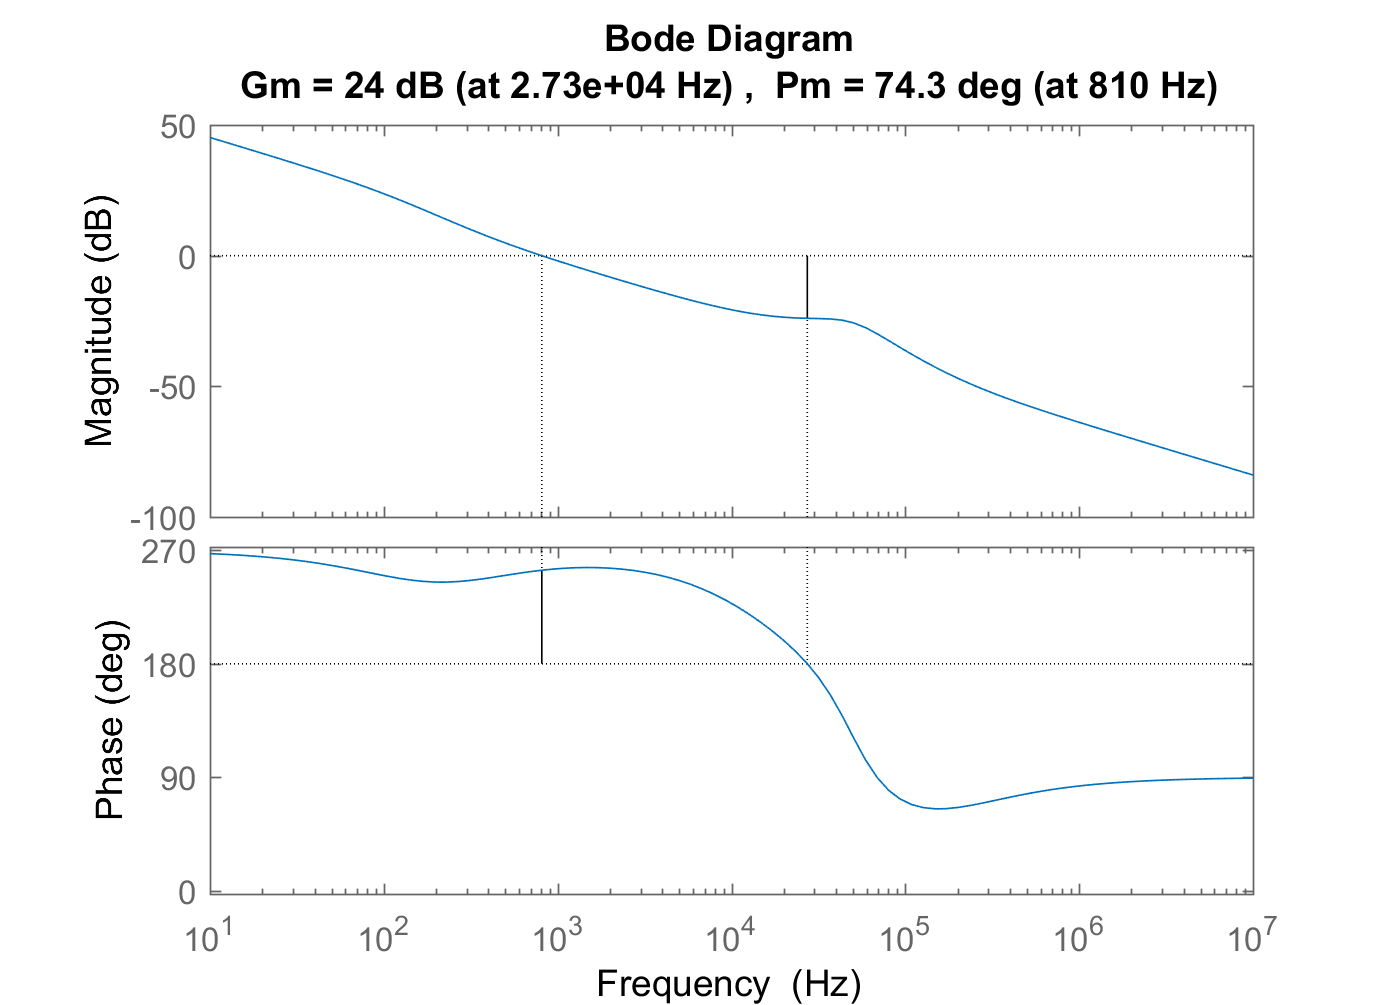
\includegraphics[max width=0.7\linewidth]{/tex/2iteration/billeder/MATLAB_total.PNG}
	\caption{Bode plot for converteren}
	\label{fig:MATLAB_total_2}
\end{figure} 


